
\chapter{Concept Model}
\label{chap:lu.uni.lassy.excalibur.group09.spec-CM}


\section{PrimaryTypes-Classes}
\subsection{Local view 12}
\label{sec:lu.uni.lassy.excalibur.group09.spec-CM-view-local-PrimaryTypes-Classes-12}
Figure \ref{fig:lu.uni.lassy.excalibur.group09.spec-CM-view-local-PrimaryTypes-Classes-12} Illustration of all the associations.



\begin{figure}[htbp] 
\label{fig:lu.uni.lassy.excalibur.group09.spec-CM}
\begin{center}
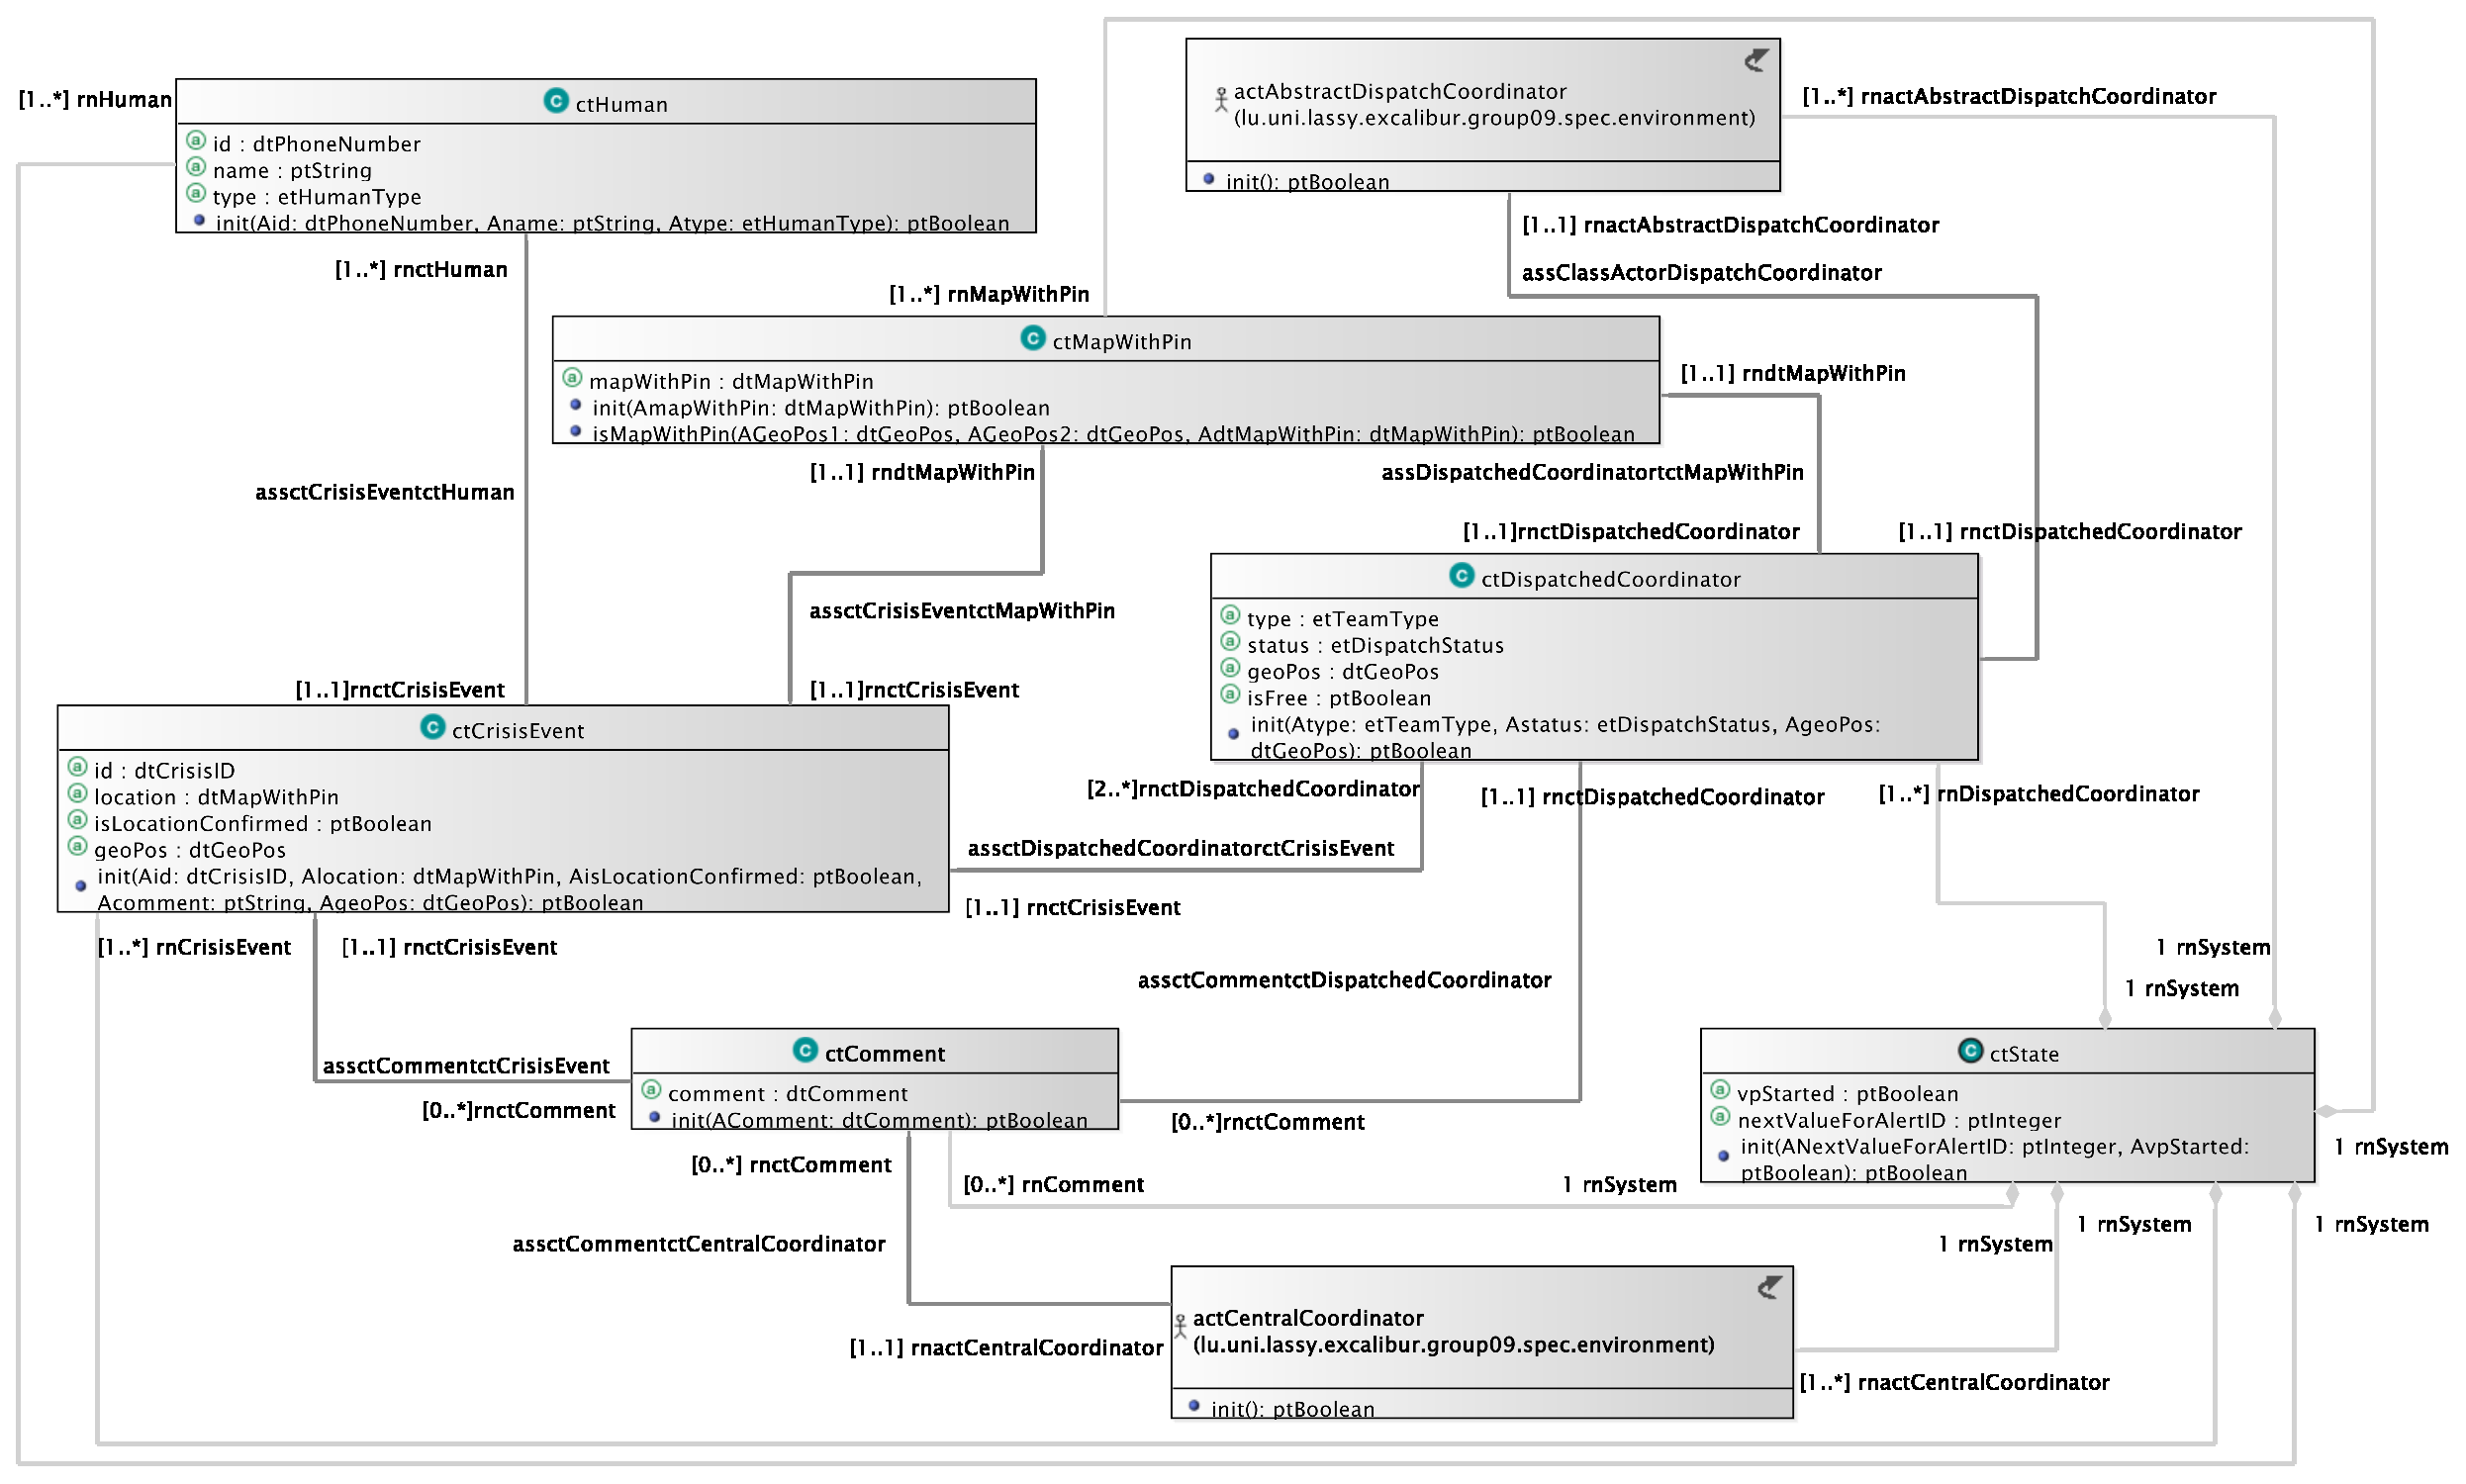
\includegraphics[
angle=90
,height=1.0\textheight
]{./images-report-gen/concept-model/local/PrimaryTypes-Classes/12/cm-ctAssociations.eps}
\end{center}
\caption[Concept Model - PrimaryTypes-Classes local view 12 - ]{Concept Model - PrimaryTypes-Classes local view 12. .}
\label{fig:lu.uni.lassy.excalibur.group09.spec-CM-view-local-PrimaryTypes-Classes-12}
\end{figure}
\vspace{0.5cm} 




\section{PrimaryTypes-Datatypes}
\subsection{Local view 01}
\label{sec:lu.uni.lassy.excalibur.group09.spec-CM-view-local-PrimaryTypes-Datatypes-01}
Figure \ref{fig:lu.uni.lassy.excalibur.group09.spec-CM-view-local-PrimaryTypes-Datatypes-01} Is representing the address data type.



\begin{figure}[htbp] 
\label{fig:lu.uni.lassy.excalibur.group09.spec-CM}
\begin{center}
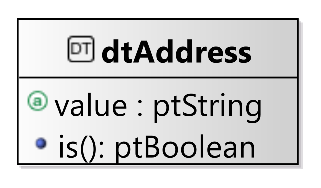
\includegraphics[
angle=0
]{./images-report-gen/concept-model/local/PrimaryTypes-Datatypes/01/cm-dtv-address.eps}
\end{center}
\caption[Concept Model - PrimaryTypes-Datatypes local view 01 - ]{Concept Model - PrimaryTypes-Datatypes local view 01. .}
\label{fig:lu.uni.lassy.excalibur.group09.spec-CM-view-local-PrimaryTypes-Datatypes-01}
\end{figure}
\vspace{0.5cm} 

\subsection{Local view 02}
\label{sec:lu.uni.lassy.excalibur.group09.spec-CM-view-local-PrimaryTypes-Datatypes-02}
Figure \ref{fig:lu.uni.lassy.excalibur.group09.spec-CM-view-local-PrimaryTypes-Datatypes-02} Is representing the crisis id data type.



\begin{figure}[htbp] 
\label{fig:lu.uni.lassy.excalibur.group09.spec-CM}
\begin{center}
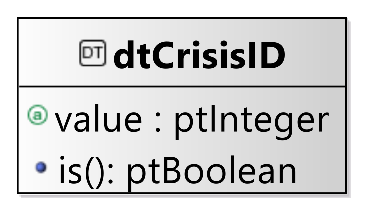
\includegraphics[
angle=0
]{./images-report-gen/concept-model/local/PrimaryTypes-Datatypes/02/cm-dtv-crisisID.eps}
\end{center}
\caption[Concept Model - PrimaryTypes-Datatypes local view 02 - ]{Concept Model - PrimaryTypes-Datatypes local view 02. .}
\label{fig:lu.uni.lassy.excalibur.group09.spec-CM-view-local-PrimaryTypes-Datatypes-02}
\end{figure}
\vspace{0.5cm} 

\subsection{Local view 03}
\label{sec:lu.uni.lassy.excalibur.group09.spec-CM-view-local-PrimaryTypes-Datatypes-03}
Figure \ref{fig:lu.uni.lassy.excalibur.group09.spec-CM-view-local-PrimaryTypes-Datatypes-03} Is representing the map including a pin data type.



\begin{figure}[htbp] 
\label{fig:lu.uni.lassy.excalibur.group09.spec-CM}
\begin{center}
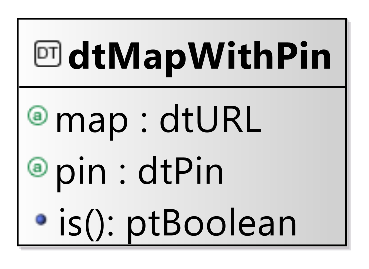
\includegraphics[
angle=0
]{./images-report-gen/concept-model/local/PrimaryTypes-Datatypes/03/cm-dtv-mapWithPin.eps}
\end{center}
\caption[Concept Model - PrimaryTypes-Datatypes local view 03 - ]{Concept Model - PrimaryTypes-Datatypes local view 03. .}
\label{fig:lu.uni.lassy.excalibur.group09.spec-CM-view-local-PrimaryTypes-Datatypes-03}
\end{figure}
\vspace{0.5cm} 

\subsection{Local view 04}
\label{sec:lu.uni.lassy.excalibur.group09.spec-CM-view-local-PrimaryTypes-Datatypes-04}
\input{doc-gen/concept-model/local/PrimaryTypes-Datatypes/04/CM-view-local-PrimaryTypes-Datatypes-04.tex}
\subsection{Local view 05}
\label{sec:lu.uni.lassy.excalibur.group09.spec-CM-view-local-PrimaryTypes-Datatypes-05}
Figure \ref{fig:lu.uni.lassy.excalibur.group09.spec-CM-view-local-PrimaryTypes-Datatypes-05} Is representing the dispatch status enumeration type.



\begin{figure}[htbp] 
\label{fig:lu.uni.lassy.excalibur.group09.spec-CM}
\begin{center}
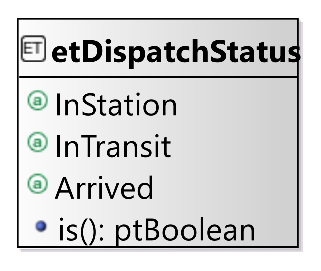
\includegraphics[
angle=0
]{./images-report-gen/concept-model/local/PrimaryTypes-Datatypes/05/cm-etv-dispatchStatus.eps}
\end{center}
\caption[Concept Model - PrimaryTypes-Datatypes local view 05 - ]{Concept Model - PrimaryTypes-Datatypes local view 05. .}
\label{fig:lu.uni.lassy.excalibur.group09.spec-CM-view-local-PrimaryTypes-Datatypes-05}
\end{figure}
\vspace{0.5cm} 

\subsection{Local view 06}
\label{sec:lu.uni.lassy.excalibur.group09.spec-CM-view-local-PrimaryTypes-Datatypes-06}
Figure \ref{fig:lu.uni.lassy.excalibur.group09.spec-CM-view-local-PrimaryTypes-Datatypes-06} Is representing the human type enumeration type.



\begin{figure}[htbp] 
\label{fig:lu.uni.lassy.excalibur.group09.spec-CM}
\begin{center}
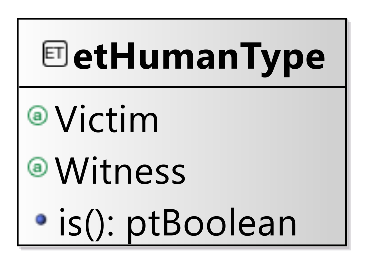
\includegraphics[
angle=0
]{./images-report-gen/concept-model/local/PrimaryTypes-Datatypes/06/cm-etv-humanType.eps}
\end{center}
\caption[Concept Model - PrimaryTypes-Datatypes local view 06 - ]{Concept Model - PrimaryTypes-Datatypes local view 06. .}
\label{fig:lu.uni.lassy.excalibur.group09.spec-CM-view-local-PrimaryTypes-Datatypes-06}
\end{figure}
\vspace{0.5cm} 

\subsection{Local view 07}
\label{sec:lu.uni.lassy.excalibur.group09.spec-CM-view-local-PrimaryTypes-Datatypes-07}
Figure \ref{fig:lu.uni.lassy.excalibur.group09.spec-CM-view-local-PrimaryTypes-Datatypes-07} Is representing the team type enumeration type.



\begin{figure}[htbp] 
\label{fig:lu.uni.lassy.excalibur.group09.spec-CM}
\begin{center}
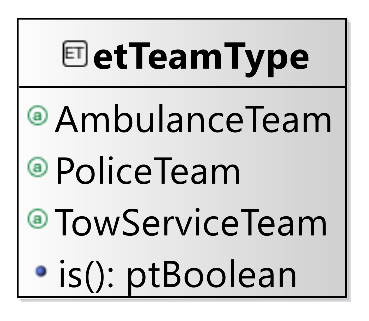
\includegraphics[
angle=0
]{./images-report-gen/concept-model/local/PrimaryTypes-Datatypes/07/cm-etv-teamType.eps}
\end{center}
\caption[Concept Model - PrimaryTypes-Datatypes local view 07 - ]{Concept Model - PrimaryTypes-Datatypes local view 07. .}
\label{fig:lu.uni.lassy.excalibur.group09.spec-CM-view-local-PrimaryTypes-Datatypes-07}
\end{figure}
\vspace{0.5cm} 










\section{Concept Model Types Descriptions}
This section provides the textual descriptions of all the types defined in the concept model and that can be part of the graphical views provided.

\subsection{Primary types - Class types descriptions}




The table below is providing comments on the graphical views given for the class types of the primary types. Type logical operations are precisely specified in the operation model.

\begin{datadictionary}
\addheading{Classes}

\adddoublerow{ctCrisisEvent}{A class containing the attributes identifying a crisis event.}
\adddoubletwocolumnrow{attribute}{\msrcode{comment: ptString}}{}
\adddoubletwocolumnrow{attribute}{\msrcode{id: ptInteger}}{}
\adddoubletwocolumnrow{attribute}{\msrcode{isLocationConfirmed: ptBoolean}}{}
\adddoubletwocolumnrow{attribute}{\msrcode{location: dtMapWithPin}}{}
\adddoubletwocolumnrow{operation}{\msrcode{init(Aid:ptInteger, Alocation:dtMapWithPin, AisLocationConfirmed:ptBoolean, Acomment:ptString, AgeoPos:dtGeoPos):ptBoolean}}{}
\adddoublerow{ctDispatchedCoordinator}{A class containing the attributes identifying a dispatched team.}
\adddoubletwocolumnrow{attribute}{\msrcode{status: etDispatchStatus}}{}
\adddoubletwocolumnrow{attribute}{\msrcode{type: etTeamType}}{}
\adddoubletwocolumnrow{operation}{\msrcode{init(Atype:etTeamType, Astatus:etDispatchStatus, AgeoPos:dtGeoPos):ptBoolean}}{}
\adddoublerow{ctHuman}{A class containing the attributes identifying an human.}
\adddoubletwocolumnrow{attribute}{\msrcode{id: dtPhoneNumber}}{}
\adddoubletwocolumnrow{attribute}{\msrcode{name: ptString}}{}
\adddoubletwocolumnrow{attribute}{\msrcode{type: etHumanType}}{}
\adddoubletwocolumnrow{operation}{\msrcode{init(Aid:dtPhoneNumber, Aname:ptString, Atype:etHumanType):ptBoolean}}{}
\adddoublerow{ctMapWithPin}{A class containing an image which is the map including the pins.}
\adddoubletwocolumnrow{attribute}{\msrcode{mapWithPin: dtMapWithPin}}{}
\adddoubletwocolumnrow{operation}{\msrcode{init(AmapWithPin:dtMapWithPin):ptBoolean}}{}
\end{datadictionary}

\subsection{Primary types - Datatypes types descriptions}





The table below is providing comments on the graphical views given for the datatype types of the primary types.


\begin{datadictionary}
\addheading{Datatypes}

\adddoublerow{dtAddress}{A string used to identify location addresses.}
\adddoubletwocolumnrow{attribute}{\msrcode{value: ptString}}{}
\adddoublerow{dtCrisisID}{An integer used to identify crisis events.}
\adddoubletwocolumnrow{attribute}{\msrcode{value: ptInteger}}{}
\adddoublerow{dtMapWithPin}{An URL including a two coordinates (real numbers) used to identify a map including a pin given by Google Maps.}
\adddoubletwocolumnrow{attribute}{\msrcode{map: dtURL}}{}
\adddoubletwocolumnrow{attribute}{\msrcode{pin: dtPin}}{}
\adddoublerow{dtPhoneNumber}{An Integer used to identify phone numbers.}
\adddoubletwocolumnrow{attribute}{\msrcode{value: ptInteger}}{}
\end{datadictionary}


\begin{datadictionary}
\addheading{Enumerations}

\adddoublerow{etDispatchStatus}{A String used to identify a dispatch status.}
\adddoublerow{etHumanType}{A String used to identify an Human type.}
\adddoublerow{etTeamType}{A String used to identify a team type.}
\end{datadictionary}






\subsection{Primary types - Association types descriptions}




The table below is providing comments on the association types of the primary types.

\begin{associationtypes}
\addheading{Undirected associations}
\adddoublerow{assClassActorDisptachCoordinator}{Association of a dispatched coordinator to an actor of the same type.}
\adddoublerow{assctCrisisEventctHuman}{Association of a crisis event to an human.}
\adddoublerow{assctDispatchedCoordinatorctCrisisEvent}{Association of a dispatched coordinator to a crisis event.}
\end{associationtypes}

\input{doc-gen/concept-model/comments-tables/primaryTypesAggregations-comments-table.tex}
\input{doc-gen/concept-model/comments-tables/primaryTypesCompositions-comments-table.tex}
\input{doc-gen/concept-model/comments-tables/secondaryTypesClasses-comments-table.tex}
\subsection{Secondary types - Datatypes types descriptions}





The table below is providing comments on the graphical views given for the datatype types of the secondary types.

\begin{datadictionary}
\addheading{Datatypes}

\adddoublerow{dtAddress}{A String used to identify an address.}
\addsingletwocolumnrow{extends}{dtString}
\adddoubletwocolumnrow{operation}{\msrcode{is():ptBoolean}}{}
\adddoublerow{dtComment}{A String used to identify a comment.}
\addsingletwocolumnrow{extends}{dtString}
\adddoubletwocolumnrow{operation}{\msrcode{is():ptBoolean}}{}
\adddoublerow{dtCrisisID}{An Integer used to identify a crisis id.}
\addsingletwocolumnrow{extends}{dtInteger}
\adddoubletwocolumnrow{operation}{\msrcode{is():ptBoolean}}{}
\adddoublerow{dtImage}{A String used to identify an image.}
\addsingletwocolumnrow{extends}{dtString}
\adddoubletwocolumnrow{operation}{\msrcode{is():ptBoolean}}{}
\adddoublerow{dtLatitude}{used to define a latitude value of a geograpical positions on earth.}
\addsingletwocolumnrow{extends}{dtReal}
\adddoubletwocolumnrow{operation}{\msrcode{is():ptBoolean}}{}
\adddoublerow{dtLongitude}{used to define a longitude value of a geograpical positions on earth.}
\addsingletwocolumnrow{extends}{dtReal}
\adddoubletwocolumnrow{operation}{\msrcode{is():ptBoolean}}{}
\adddoublerow{dtMapWithPin}{An image which is a map including pins.}
\addsingletwocolumnrow{extends}{dtImage}
\adddoubletwocolumnrow{operation}{\msrcode{is():ptBoolean}}{}
\adddoublerow{dtPhoneNumber}{A String used to store a phone number.}
\addsingletwocolumnrow{extends}{dtString}
\adddoubletwocolumnrow{operation}{\msrcode{is():ptBoolean}}{}
\end{datadictionary}





\input{doc-gen/concept-model/comments-tables/secondaryTypesAssociations-comments-table.tex}
\input{doc-gen/concept-model/comments-tables/secondaryTypesAggregations-comments-table.tex}
\input{doc-gen/concept-model/comments-tables/secondaryTypesCompositions-comments-table.tex}

